\section{Architectures}
Different type of architectures are available depending on the speed and power constraints.
To fulfill desired specifications the following optimizations can be done:\\
\begin{itemize}
    \item Reduce total number of operations, in particular multiplications that are heavier
    \item Fixed-point arithmetic is cheaper and faster
    \item The area of a fixed point parallel multiplier is proportional to the product of the coefficient and data word lengths one could try to reduce their word length
\end{itemize}
Suppose a filter of order N has to be realized.
\subsection{Direct form}
This structure requires N memory locations for storing previous inputs and in terms of complexity it does N+1 multiplications and  N additions.  For building this structure the definition of Equation \ref{eq:general} is used to derive the equivalent circuit.
\begin{figure}[H]
    \centering
    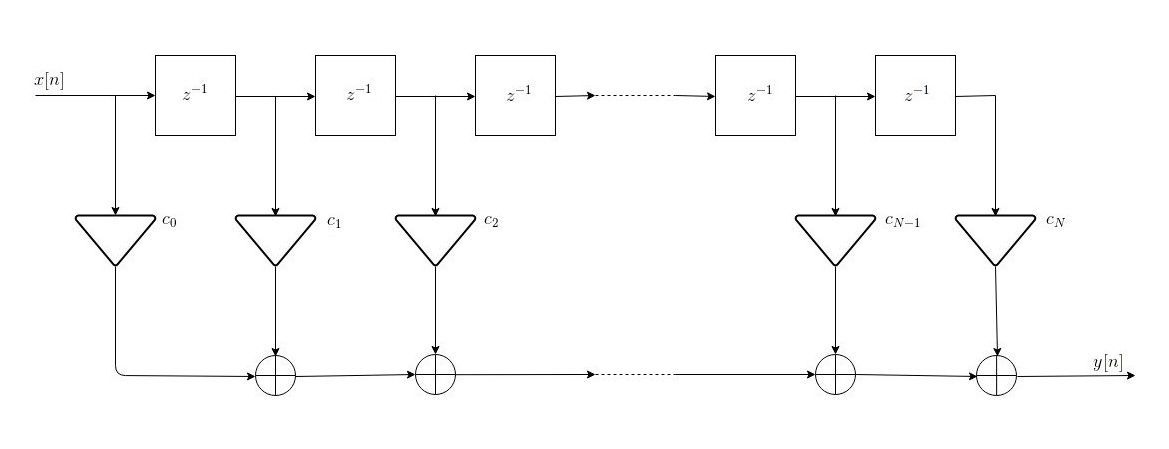
\includegraphics[scale=0.45]{images/direct.jpeg}    
    \caption{scheme of direct form}
    \label{fig:my_label}
\end{figure}
\subsection{Transposed form}
This structure is very similar at first look w.r.t. the previous one but in the former there was a big addition in the end, here instead there is a set of small additions separated by delay elements.
\begin{figure}[H]
    \centering
    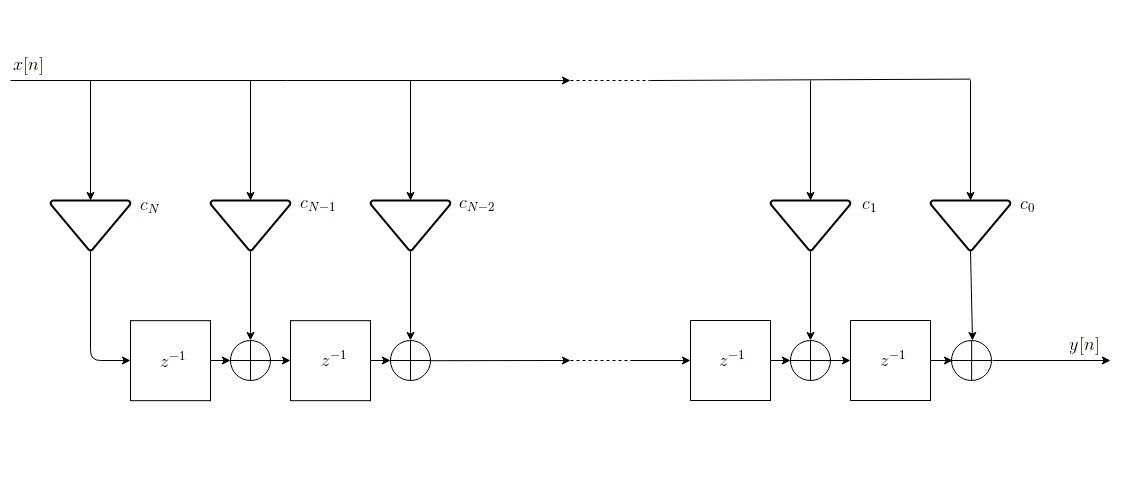
\includegraphics[scale=0.45]{images/transposed.jpg}    
    \caption{scheme of transposed form}
    \label{fig:transposed}
\end{figure}
\subsection{Symmetric taps (linear phase)}
FIR filters are often designed to have symmetry in the filter taps so exploit this symmetry can be exploited in order to reduce the number of multiplications.
$$y[n]= c_{0}(x[n]+x[0])+c_{1}(x[n-1]+x[1])+....+c_{N/2}(x[N/2])$$
The last term of the previous equation is needed only if N is even.
With this type of implementation the number of multiplications is reduced to $\left \lfloor N/2+1 \right \rfloor$
\begin{figure}[H]
    \centering
    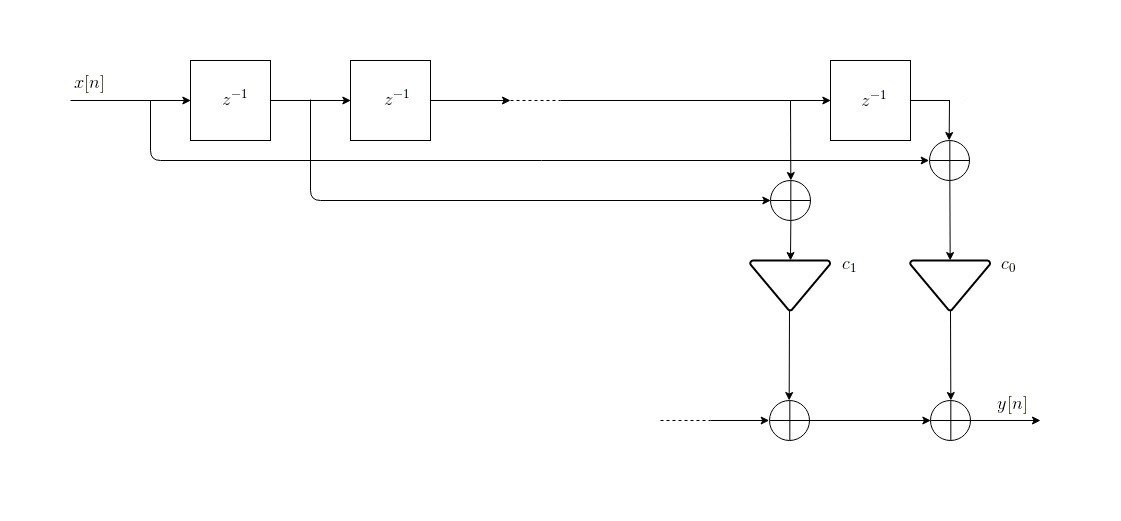
\includegraphics[scale=0.45]{images/symmetryc.jpg}    
    \caption{direct form with symmetric taps}
    \label{fig:symmetric}
\end{figure}
\subsection{Cascade form}
The transfer function is expressed as product of second-order polynomial system functions via factorization:
\begin{equation} \label{eq:1}
H(z)=\frac{y[n]}{x[n]} =\sum_{i=0}^{N}c_{i}z^{-i}= \prod_{i=1}^{M_{c}}(\beta_{0i}+\beta_{1i}z^{-1}+\beta_{2i}z^{-2})
\end{equation}
Where $M_{c}= \left \lfloor (N+1)/2 \right \rfloor$.
Assuming that N is even, this implementation needs N storage elements, $\frac{3N}{2}$ multiplications and N additions for each output value.
\begin{figure}[H]
    \centering
    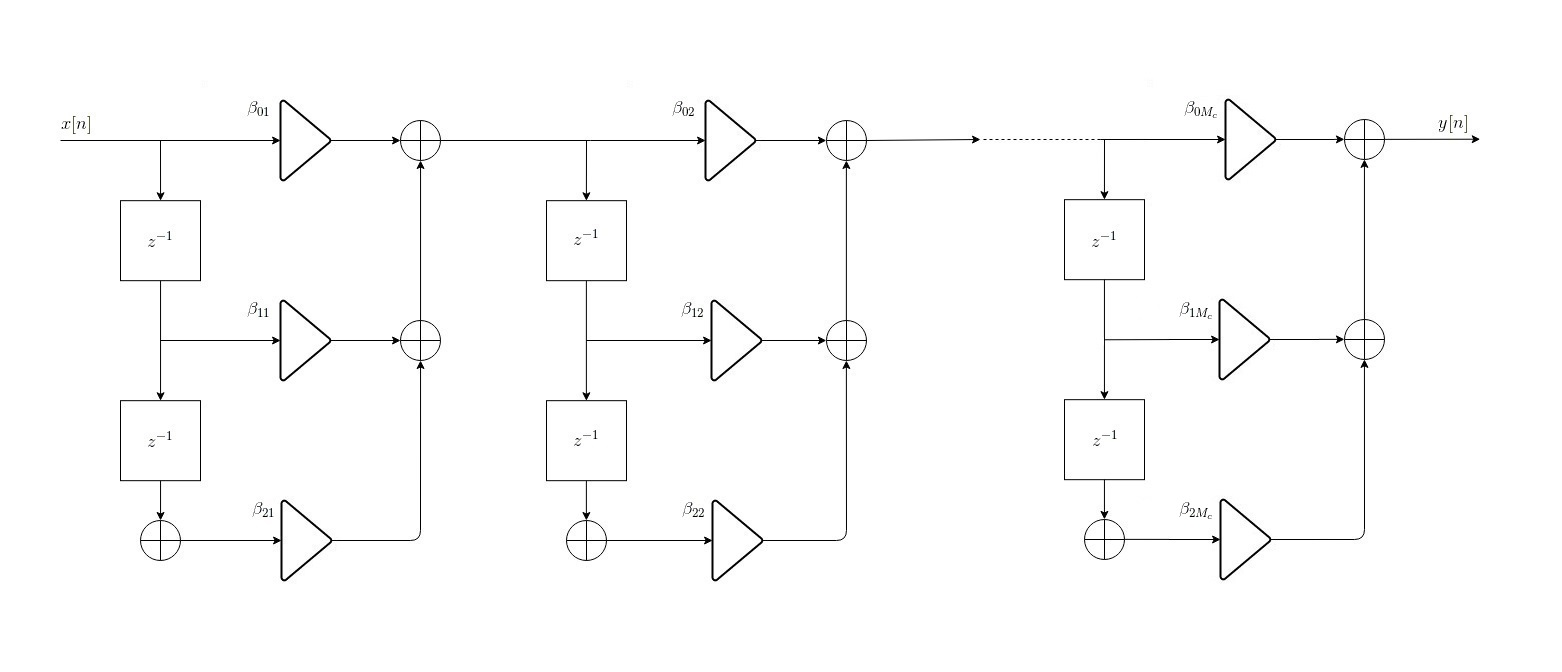
\includegraphics[scale=0.35]{images/cascade.jpg}    
    \caption{cascade form}
    \label{fig:cascade}
\end{figure}
To save computational complexity, Equation (\ref{eq:1}) is expressed as:
\begin{equation} \label{eq:2}
H(z)= G\prod_{i=1}^{M_{c}}(1+\beta_{1i}'z^{-1}+\beta_{2i}'z^{-2})
\end{equation}
where $G=\beta_{01}\beta_{02} \cdot\cdot\cdot\beta_{0M_{c}}$ ,$\beta_{1i}'=\beta_{1i}/\beta_{0i}$ , $i= 1,2,\cdot \cdot \cdot,M_{c}$ in this way all $\beta_{0i}$ are normalized to 1 as one can see in (Equation \ref{eq:2}). Assuming that N is even N delay elements are needed, (N+1) multiplications and N additions, for computing each output value.
\begin{figure}[H]
    \centering
    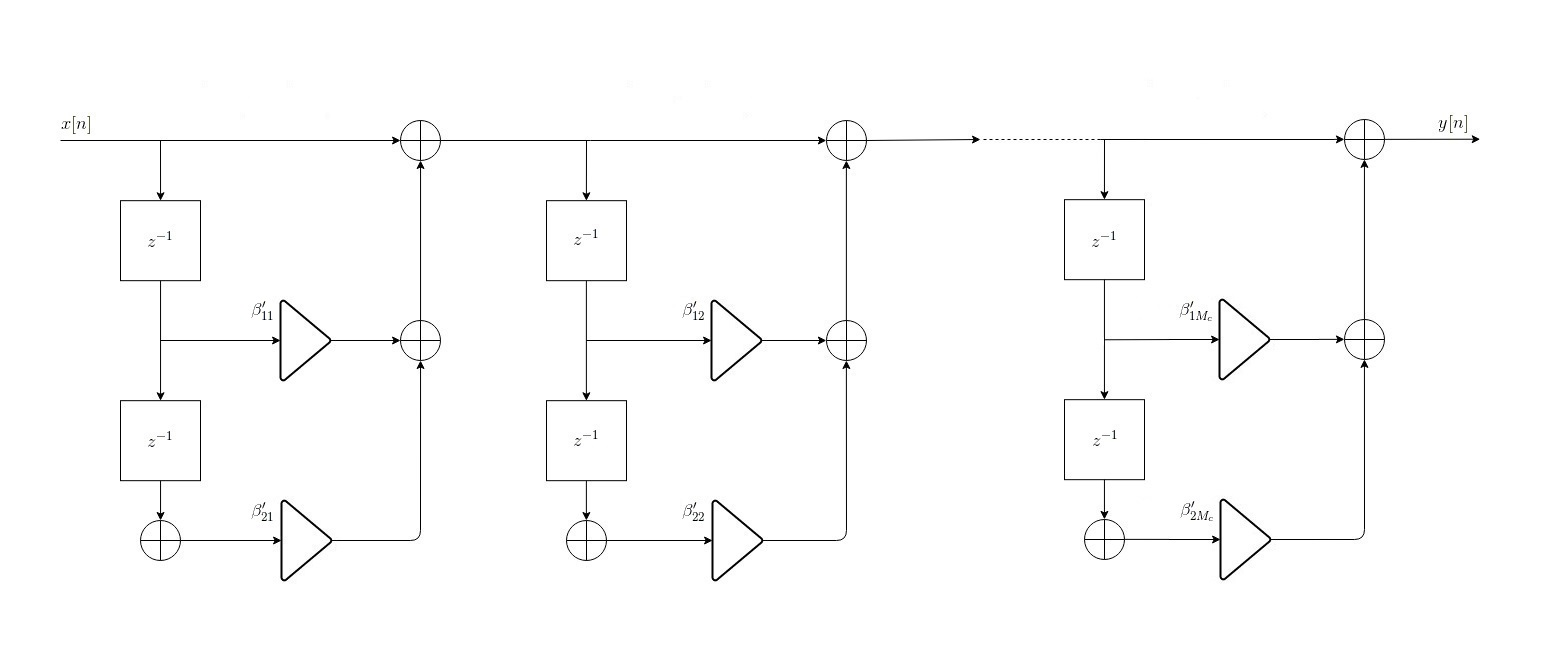
\includegraphics[scale=0.35]{images/cascadeoptimised.jpg}    
    \caption{cascade form with lower complexity}
    \label{fig:cascade_opt}
\end{figure}
